\documentclass[../main.tex]{subfiles}

\begin{document}


\subsection{Resumen de actividades}

Durante el semestre se trabajó principalmente en realizar correcciones al protocolo de simulaciones y realizar simulaciones de prueba con el protocolo correguido.
Las principales correcciones que se realizaron fueron:
\begin{enumerate}
    \item Correguir la implmentación del potencial de 3 cuerpos en LAMMPS
    \item Cambiar el comando \texttt{write\_data} por el comando \texttt{restart}.
    \item Adaptar el promedio temporal de los commandos \texttt{fix} para los observables de energía y estrés.
    \item Corrección en el cálculo de densidad de empaquetamiento de las simulaciones.
\end{enumerate}
Por otro lado las simulaciones de pruebas fueron realizandose para ir monitoreando que las comabios realizados no alteraran significativamente el comportamiento cualitativo esperado de las relaciones entre deformación y estrés.

Una vez que se implementaron todas las correcciones, se empezaron a realizar simulaciones de exploración de parametros con el objetivo de ir analizando el sistema.
Los parámetros que se variaron fueron el ritmo de deformación y el \texttt{damp}.

\subsection{Resultados principales}

En esta sección se presentan los resultados obtenidos con el protocolo de simulación correguido.
Las simulaciones se realizaron en sistemas de \num{8000} partículas con \num{3}\% de partículas con 4 patches.
Los resultados principales que se presetan son la relación preliminar entre el ritmo de deformación con la componente en dirección de deformación del estrés virial en estado estacionario durante una deformación de cizallamiento (figura~\ref{fig:shear-rate-vs-stress}) y la evolución del estrés virial durante una deformación de cizallamiento (figura~\ref{fig:strain-vs-stress}), junto con las correcciones realizadas en el protocolo de simulación con un valor de damp igual a \num{0.1}.

En la figura~\ref{fig:shear-rate-vs-stress} se observa que el estrés durante el estado estacionario va incrementando conforme el rito de deformación va aumentando, asegurandonos que las correcciones mantienen el comportamiento esperado.
Por otro lado, se especula que a ritmos más bajos de deformación, la tendencia es hacia un estrés en estado estacionario casi nulo, lo cuál indicaría que el modelo para el hidrogel que se está usando no es adecuado para explorar propiedades reológicas de hidrogeles.
Sin embargo, si es posible usar este modelo para explorar la conexión entre la respuesta mecánica de sistemas que tienen la capacidad de re-configurar todos sus enlaces durante una deformación.

\begin{figure}[h]
    \centering
    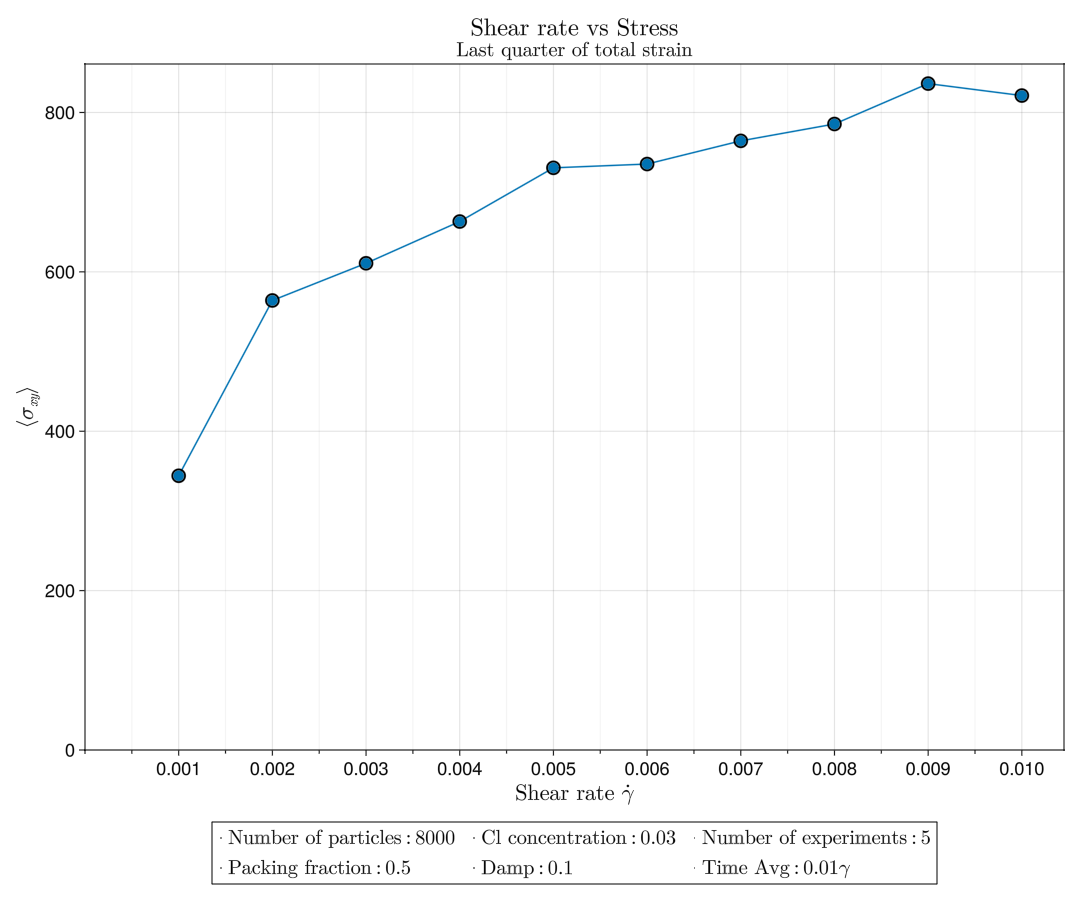
\includegraphics[width=0.9\textwidth]{../Figures/system-2025-05-22-194804-CL-0.03/ShearRate-vs-Stress.png}
    \caption{Promedio de la componente $xy$ del tensor de estrés virial en estado estacionario para distintos ritmos de deformación.}\label{fig:shear-rate-vs-stress}
\end{figure}

En la figura~\ref{fig:strain-vs-stress} se puede observar un máximo de estrés durante el inicio del proceso de cizallamiento y un proceso de equilibrio en un lapso de aproximadamente $5\gamma$. 
Posteriormente, al continuar con la deformación, encontramos que el estrés tiende a no variar mucho cuando la deformación llega a $\gamma>12$, por lo que se decidio usar esos valores en adelante para crear el promedio del estrés en estado estacionario de la figura~\ref{fig:shear-rate-vs-stress}.

\begin{figure}[h]
    \centering
    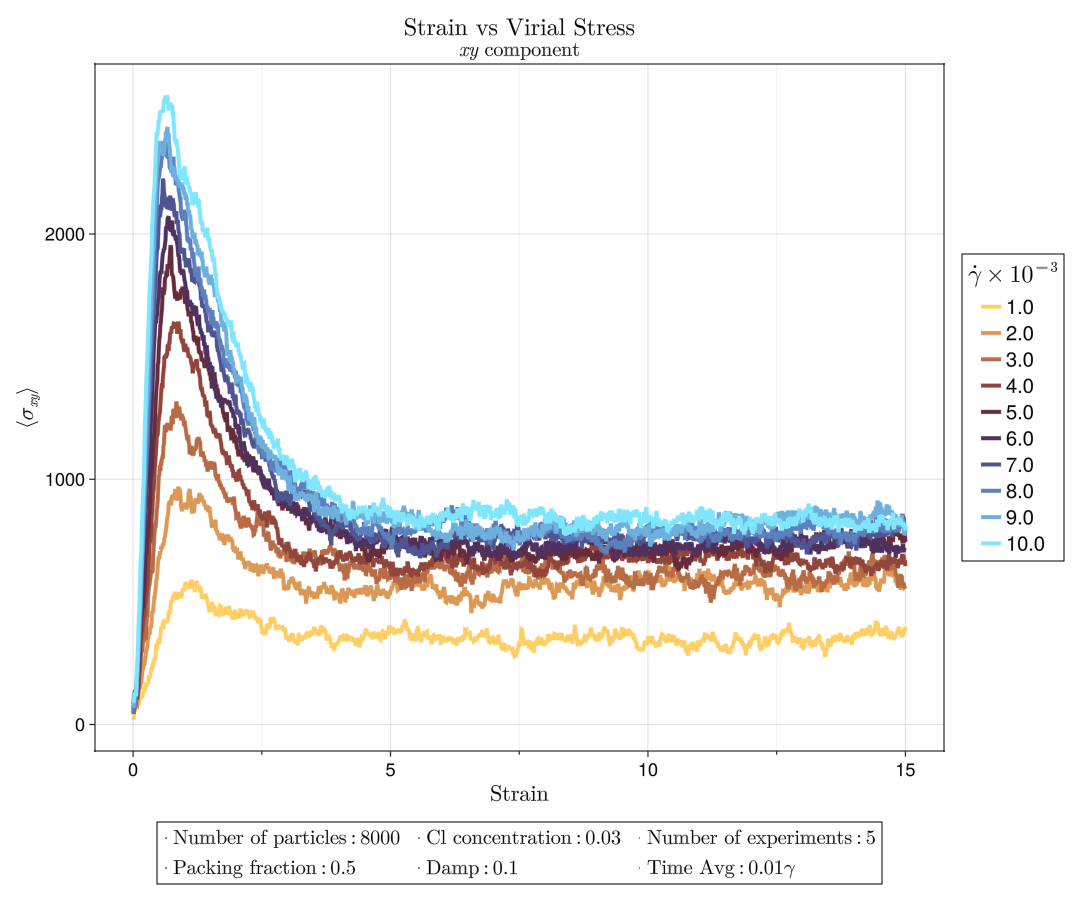
\includegraphics[width=0.9\textwidth]{../Figures/system-2025-05-22-194804-CL-0.03/Strain-vs-StressVirialXY.png}
    \caption{Promedio temporal de la component $xy$ del tensor de estrés virial durante una deformación de tipo cizallamiento para distintos ritmos de deformación.}\label{fig:strain-vs-stress}
\end{figure}

\subsection{Resultados generales}

Otro resultado interesante de la relación observada en la figura~\ref{fig:strain-vs-stress} es el desplazamiento del estrés máximo hacia menores $\gamma$ cuando el ritmo de deformación aumenta, está tendencia se puede observar claramente en la figura~\ref{fig:Zoomstrain-vs-stress}.
También se observa que al ir incrementando el ritmo de deformación el valor máximo aumenta proporcionalmente.

\begin{figure}[h]
    \centering
    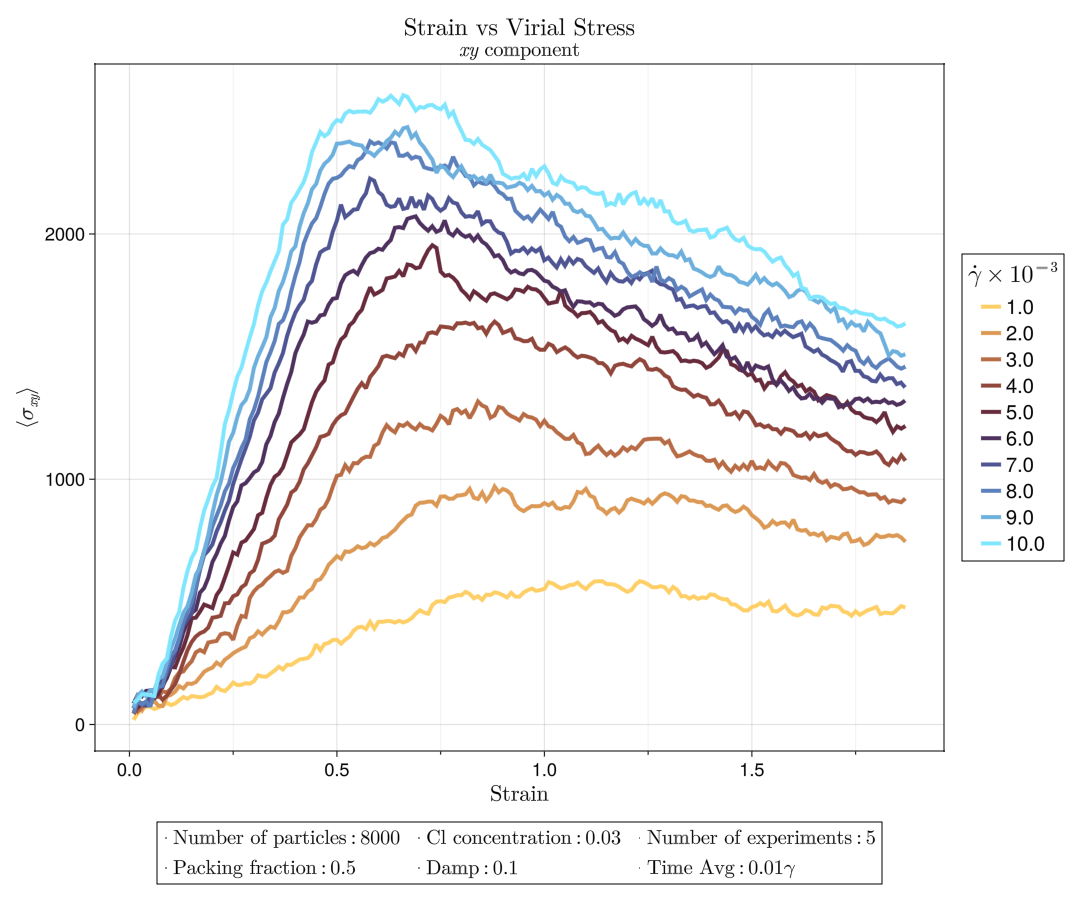
\includegraphics[width=0.9\textwidth]{../Figures/system-2025-05-22-194804-CL-0.03/Strain-vs-Stress-Zoom.png}
    \caption{Promedio temporal de la component $xy$ del tensor de estrés virial durante el inicio de una deformación de tipo cizallamiento para distintos ritmos de deformación}\label{fig:Zoomstrain-vs-stress}
\end{figure}

\begin{figure}[h]
    \centering
    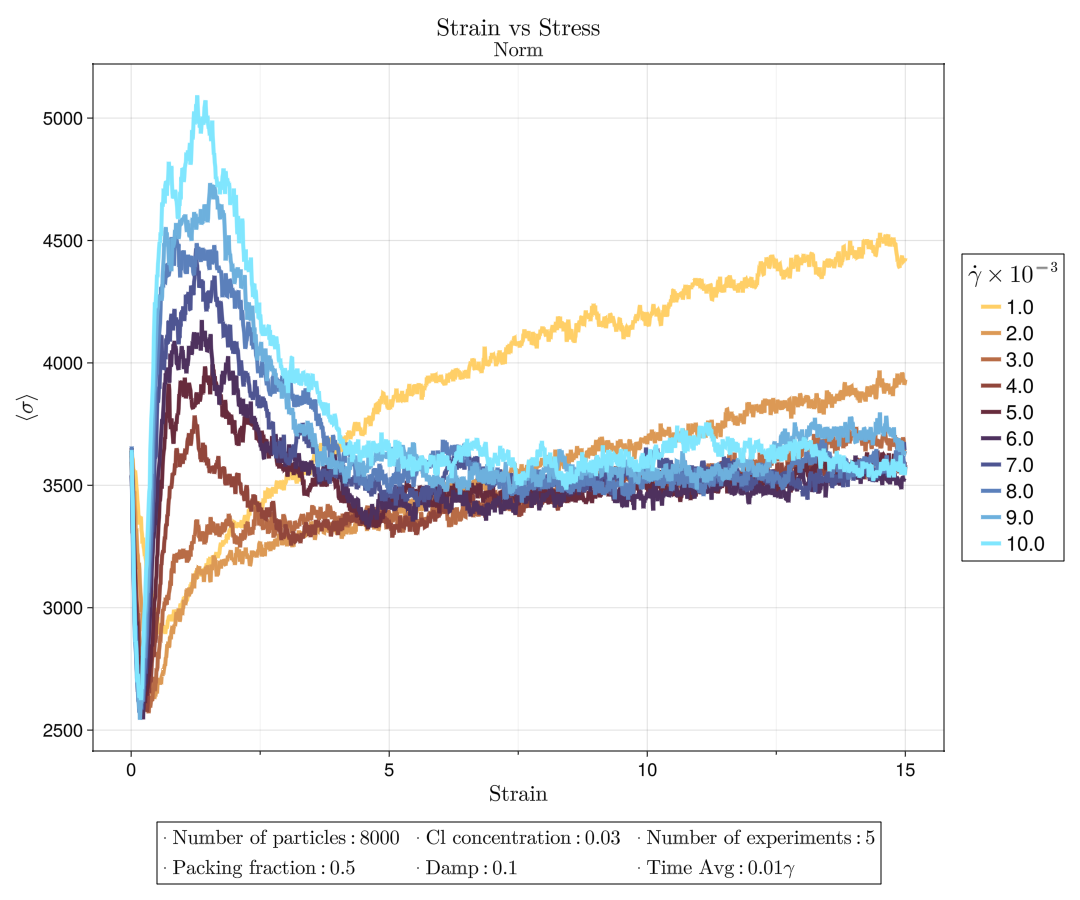
\includegraphics[width=0.9\textwidth]{../Figures/system-2025-05-22-194804-CL-0.03/Strain-vs-StressNORM.png}
    \caption{Promedio temporal de la norma del tensor de estrés durante una deformación de tipo cizallamiento para distintos ritmos de deformación}\label{fig:strain-vs-normstress}
\end{figure}

Por último, tambén se analizó la evolución temporal de la norma del tensor de estrés durante la deformación (figura~\ref{fig:strain-vs-normstress}) y al comparar los ordenes de magnitud y el comportamiento cualitativo de la evolución temporal mostrada con la figura~\ref{fig:strain-vs-stress}, podemos observar que la principal contribución al comportamiento cualitativo de la norma del estrés en ritmos de deformación mayores a $3$, surge de la componente del término virial alineada en la dirección de deformación, permitiendo sugerir que la respuesta mecánica está fuertemente influenciada por los potenciales de interacción entre las partículas patchy.


\end{document}
